\documentclass[1p]{elsarticle_modified}
%\bibliographystyle{elsarticle-num}

%\usepackage[colorlinks]{hyperref}
%\usepackage{abbrmath_seonhwa} %\Abb, \Ascr, \Acal ,\Abf, \Afrak
\usepackage{amsfonts}
\usepackage{amssymb}
\usepackage{amsmath}
\usepackage{amsthm}
\usepackage{scalefnt}
\usepackage{amsbsy}
\usepackage{kotex}
\usepackage{caption}
\usepackage{subfig}
\usepackage{color}
\usepackage{graphicx}
\usepackage{xcolor} %% white, black, red, green, blue, cyan, magenta, yellow
\usepackage{float}
\usepackage{setspace}
\usepackage{hyperref}

\usepackage{tikz}
\usetikzlibrary{arrows}

\usepackage{multirow}
\usepackage{array} % fixed length table
\usepackage{hhline}

%%%%%%%%%%%%%%%%%%%%%
\makeatletter
\renewcommand*\env@matrix[1][\arraystretch]{%
	\edef\arraystretch{#1}%
	\hskip -\arraycolsep
	\let\@ifnextchar\new@ifnextchar
	\array{*\c@MaxMatrixCols c}}
\makeatother %https://tex.stackexchange.com/questions/14071/how-can-i-increase-the-line-spacing-in-a-matrix
%%%%%%%%%%%%%%%

\usepackage[normalem]{ulem}

\newcommand{\msout}[1]{\ifmmode\text{\sout{\ensuremath{#1}}}\else\sout{#1}\fi}
%SOURCE: \msout is \stkout macro in https://tex.stackexchange.com/questions/20609/strikeout-in-math-mode

\newcommand{\cancel}[1]{
	\ifmmode
	{\color{red}\msout{#1}}
	\else
	{\color{red}\sout{#1}}
	\fi
}

\newcommand{\add}[1]{
	{\color{blue}\uwave{#1}}
}

\newcommand{\replace}[2]{
	\ifmmode
	{\color{red}\msout{#1}}{\color{blue}\uwave{#2}}
	\else
	{\color{red}\sout{#1}}{\color{blue}\uwave{#2}}
	\fi
}

\newcommand{\Sol}{\mathcal{S}} %segment
\newcommand{\D}{D} %diagram
\newcommand{\A}{\mathcal{A}} %arc


%%%%%%%%%%%%%%%%%%%%%%%%%%%%%5 test

\def\sl{\operatorname{\textup{SL}}(2,\Cbb)}
\def\psl{\operatorname{\textup{PSL}}(2,\Cbb)}
\def\quan{\mkern 1mu \triangleright \mkern 1mu}

\theoremstyle{definition}
\newtheorem{thm}{Theorem}[section]
\newtheorem{prop}[thm]{Proposition}
\newtheorem{lem}[thm]{Lemma}
\newtheorem{ques}[thm]{Question}
\newtheorem{cor}[thm]{Corollary}
\newtheorem{defn}[thm]{Definition}
\newtheorem{exam}[thm]{Example}
\newtheorem{rmk}[thm]{Remark}
\newtheorem{alg}[thm]{Algorithm}

\newcommand{\I}{\sqrt{-1}}
\begin{document}

%\begin{frontmatter}
%
%\title{Boundary parabolic representations of knots up to 8 crossings}
%
%%% Group authors per affiliation:
%\author{Yunhi Cho} 
%\address{Department of Mathematics, University of Seoul, Seoul, Korea}
%\ead{yhcho@uos.ac.kr}
%
%
%\author{Seonhwa Kim} %\fnref{s_kim}}
%\address{Center for Geometry and Physics, Institute for Basic Science, Pohang, 37673, Korea}
%\ead{ryeona17@ibs.re.kr}
%
%\author{Hyuk Kim}
%\address{Department of Mathematical Sciences, Seoul National University, Seoul 08826, Korea}
%\ead{hyukkim@snu.ac.kr}
%
%\author{Seokbeom Yoon}
%\address{Department of Mathematical Sciences, Seoul National University, Seoul, 08826,  Korea}
%\ead{sbyoon15@snu.ac.kr}
%
%\begin{abstract}
%We find all boundary parabolic representation of knots up to 8 crossings.
%
%\end{abstract}
%\begin{keyword}
%    \MSC[2010] 57M25 
%\end{keyword}
%
%\end{frontmatter}

%\linenumbers
%\tableofcontents
%
\newcommand\colored[1]{\textcolor{white}{\rule[-0.35ex]{0.8em}{1.4ex}}\kern-0.8em\color{red} #1}%
%\newcommand\colored[1]{\textcolor{white}{ #1}\kern-2.17ex	\textcolor{white}{ #1}\kern-1.81ex	\textcolor{white}{ #1}\kern-2.15ex\color{red}#1	}

{\Large $\underline{12n_{0779}~(K12n_{0779})}$}

\setlength{\tabcolsep}{10pt}
\renewcommand{\arraystretch}{1.6}
\vspace{1cm}\begin{tabular}{m{100pt}>{\centering\arraybackslash}m{274pt}}
\multirow{5}{120pt}{
	\centering
	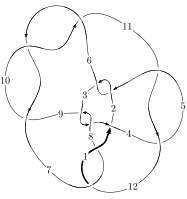
\includegraphics[width=112pt]{../../../GIT/diagram.site/Diagrams/png/2868_12n_0779.png}\\
\ \ \ A knot diagram\footnotemark}&
\allowdisplaybreaks
\textbf{Linearized knot diagam} \\
\cline{2-2}
 &
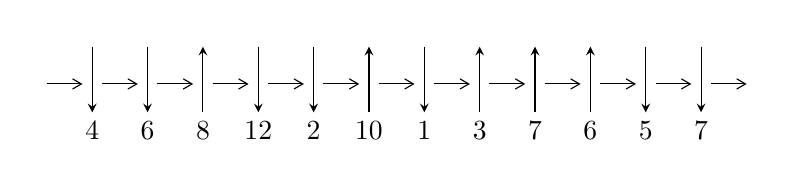
\begin{tikzpicture}[x=20pt, y=17pt]
	% nodes
	\node (C0) at (0, 0) {};
	\node (C1) at (1, 0) {};
	\node (C1U) at (1, +1) {};
	\node (C1D) at (1, -1) {4};

	\node (C2) at (2, 0) {};
	\node (C2U) at (2, +1) {};
	\node (C2D) at (2, -1) {6};

	\node (C3) at (3, 0) {};
	\node (C3U) at (3, +1) {};
	\node (C3D) at (3, -1) {8};

	\node (C4) at (4, 0) {};
	\node (C4U) at (4, +1) {};
	\node (C4D) at (4, -1) {12};

	\node (C5) at (5, 0) {};
	\node (C5U) at (5, +1) {};
	\node (C5D) at (5, -1) {2};

	\node (C6) at (6, 0) {};
	\node (C6U) at (6, +1) {};
	\node (C6D) at (6, -1) {10};

	\node (C7) at (7, 0) {};
	\node (C7U) at (7, +1) {};
	\node (C7D) at (7, -1) {1};

	\node (C8) at (8, 0) {};
	\node (C8U) at (8, +1) {};
	\node (C8D) at (8, -1) {3};

	\node (C9) at (9, 0) {};
	\node (C9U) at (9, +1) {};
	\node (C9D) at (9, -1) {7};

	\node (C10) at (10, 0) {};
	\node (C10U) at (10, +1) {};
	\node (C10D) at (10, -1) {6};

	\node (C11) at (11, 0) {};
	\node (C11U) at (11, +1) {};
	\node (C11D) at (11, -1) {5};

	\node (C12) at (12, 0) {};
	\node (C12U) at (12, +1) {};
	\node (C12D) at (12, -1) {7};
	\node (C13) at (13, 0) {};

	% arrows
	\draw[->,>={angle 60}]
	(C0) edge (C1) (C1) edge (C2) (C2) edge (C3) (C3) edge (C4) (C4) edge (C5) (C5) edge (C6) (C6) edge (C7) (C7) edge (C8) (C8) edge (C9) (C9) edge (C10) (C10) edge (C11) (C11) edge (C12) (C12) edge (C13) ;	\draw[->,>=stealth]
	(C1U) edge (C1D) (C2U) edge (C2D) (C3D) edge (C3U) (C4U) edge (C4D) (C5U) edge (C5D) (C6D) edge (C6U) (C7U) edge (C7D) (C8D) edge (C8U) (C9D) edge (C9U) (C10D) edge (C10U) (C11U) edge (C11D) (C12U) edge (C12D) ;
	\end{tikzpicture} \\
\hhline{~~} \\& 
\textbf{Solving Sequence} \\ \cline{2-2} 
 &
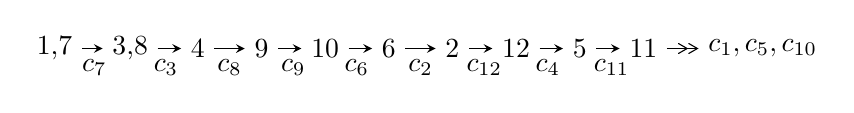
\begin{tikzpicture}[x=23pt, y=7pt]
	% node
	\node (A0) at (-1/8, 0) {1,7};
	\node (A1) at (17/16, 0) {3,8};
	\node (A2) at (17/8, 0) {4};
	\node (A3) at (25/8, 0) {9};
	\node (A4) at (33/8, 0) {10};
	\node (A5) at (41/8, 0) {6};
	\node (A6) at (49/8, 0) {2};
	\node (A7) at (57/8, 0) {12};
	\node (A8) at (65/8, 0) {5};
	\node (A9) at (73/8, 0) {11};
	\node (C1) at (1/2, -1) {$c_{7}$};
	\node (C2) at (13/8, -1) {$c_{3}$};
	\node (C3) at (21/8, -1) {$c_{8}$};
	\node (C4) at (29/8, -1) {$c_{9}$};
	\node (C5) at (37/8, -1) {$c_{6}$};
	\node (C6) at (45/8, -1) {$c_{2}$};
	\node (C7) at (53/8, -1) {$c_{12}$};
	\node (C8) at (61/8, -1) {$c_{4}$};
	\node (C9) at (69/8, -1) {$c_{11}$};
	\node (A10) at (11, 0) {$c_{1},c_{5},c_{10}$};

	% edge
	\draw[->,>=stealth]	
	(A0) edge (A1) (A1) edge (A2) (A2) edge (A3) (A3) edge (A4) (A4) edge (A5) (A5) edge (A6) (A6) edge (A7) (A7) edge (A8) (A8) edge (A9) ;
	\draw[->>,>={angle 60}]	
	(A9) edge (A10);
\end{tikzpicture} \\ 

\end{tabular} \\

\footnotetext{
The image of knot diagram is generated by the software ``\textbf{Draw programme}" developed by Andrew Bartholomew(\url{http://www.layer8.co.uk/maths/draw/index.htm\#Running-draw}), where we modified some parts for our purpose(\url{https://github.com/CATsTAILs/LinksPainter}).
}\phantom \\ \newline 
\centering \textbf{Ideals for irreducible components\footnotemark of $X_{\text{par}}$} 
 
\begin{align*}
I^u_{1}&=\langle 
4.22623\times10^{207} u^{76}+2.11947\times10^{207} u^{75}+\cdots+3.97389\times10^{208} b-1.15646\times10^{210},\\
\phantom{I^u_{1}}&\phantom{= \langle  }-9.18608\times10^{208} u^{76}+1.21921\times10^{209} u^{75}+\cdots+1.80256\times10^{210} a+1.78378\times10^{212},\\
\phantom{I^u_{1}}&\phantom{= \langle  }u^{77}- u^{76}+\cdots-8509 u+567\rangle \\
I^u_{2}&=\langle 
-457890480 u^{16}+960770667 u^{15}+\cdots+1926974837 b-992799855,\\
\phantom{I^u_{2}}&\phantom{= \langle  }702672418 u^{16}-1377478673 u^{15}+\cdots+1926974837 a+650328159,\;u^{17}- u^{16}+\cdots-4 u^2-1\rangle \\
I^u_{3}&=\langle 
10 a^3-22 a^2+93 b-35 a-73,\;2 a^4-4 a^3+7 a^2-16 a+38,\;u+1\rangle \\
I^u_{4}&=\langle 
b+1,\;a,\;u-1\rangle \\
\\
\end{align*}
\raggedright * 4 irreducible components of $\dim_{\mathbb{C}}=0$, with total 99 representations.\\
\footnotetext{All coefficients of polynomials are rational numbers. But the coefficients are sometimes approximated in decimal forms when there is not enough margin.}
\newpage
\renewcommand{\arraystretch}{1}
\centering \section*{I. $I^u_{1}= \langle 4.23\times10^{207} u^{76}+2.12\times10^{207} u^{75}+\cdots+3.97\times10^{208} b-1.16\times10^{210},\;-9.19\times10^{208} u^{76}+1.22\times10^{209} u^{75}+\cdots+1.80\times10^{210} a+1.78\times10^{212},\;u^{77}- u^{76}+\cdots-8509 u+567 \rangle$}
\flushleft \textbf{(i) Arc colorings}\\
\begin{tabular}{m{7pt} m{180pt} m{7pt} m{180pt} }
\flushright $a_{1}=$&$\begin{pmatrix}0\\u\end{pmatrix}$ \\
\flushright $a_{7}=$&$\begin{pmatrix}1\\0\end{pmatrix}$ \\
\flushright $a_{3}=$&$\begin{pmatrix}0.0509614 u^{76}-0.0676378 u^{75}+\cdots+1110.35 u-98.9581\\-0.106350 u^{76}-0.0533348 u^{75}+\cdots-389.322 u+29.1014\end{pmatrix}$ \\
\flushright $a_{8}=$&$\begin{pmatrix}1\\u^2\end{pmatrix}$ \\
\flushright $a_{4}=$&$\begin{pmatrix}0.0271559 u^{76}-0.0759271 u^{75}+\cdots+891.819 u-79.3123\\-0.134886 u^{76}-0.0541166 u^{75}+\cdots-648.919 u+47.2992\end{pmatrix}$ \\
\flushright $a_{9}=$&$\begin{pmatrix}0.178718 u^{76}+0.0499083 u^{75}+\cdots+593.550 u-12.1865\\0.0572808 u^{76}-0.0573505 u^{75}+\cdots+977.930 u-74.5360\end{pmatrix}$ \\
\flushright $a_{10}=$&$\begin{pmatrix}0.235999 u^{76}-0.00744223 u^{75}+\cdots+1571.48 u-86.7225\\0.0572808 u^{76}-0.0573505 u^{75}+\cdots+977.930 u-74.5360\end{pmatrix}$ \\
\flushright $a_{6}=$&$\begin{pmatrix}0.0765354 u^{76}+0.0880012 u^{75}+\cdots-300.208 u+26.0873\\0.241208 u^{76}+0.00575286 u^{75}+\cdots+1604.13 u-113.055\end{pmatrix}$ \\
\flushright $a_{2}=$&$\begin{pmatrix}-0.218018 u^{76}-0.108112 u^{75}+\cdots-529.500 u+20.8711\\-0.377977 u^{76}-0.0124606 u^{75}+\cdots-2608.00 u+184.881\end{pmatrix}$ \\
\flushright $a_{12}=$&$\begin{pmatrix}u\\u\end{pmatrix}$ \\
\flushright $a_{5}=$&$\begin{pmatrix}0.130908 u^{76}-0.113468 u^{75}+\cdots+1993.17 u-158.823\\-0.0311338 u^{76}-0.0916577 u^{75}+\cdots+452.432 u-32.2120\end{pmatrix}$ \\
\flushright $a_{11}=$&$\begin{pmatrix}-0.102566 u^{76}+0.101738 u^{75}+\cdots-1707.65 u+138.806\\-0.115613 u^{76}+0.0703324 u^{75}+\cdots-1447.07 u+102.159\end{pmatrix}$\\&\end{tabular}
\flushleft \textbf{(ii) Obstruction class $= -1$}\\~\\
\flushleft \textbf{(iii) Cusp Shapes $= -0.120770 u^{76}+0.0653085 u^{75}+\cdots-1789.94 u+132.110$}\\~\\
\newpage\renewcommand{\arraystretch}{1}
\flushleft \textbf{(iv) u-Polynomials at the component}\newline \\
\begin{tabular}{m{50pt}|m{274pt}}
Crossings & \hspace{64pt}u-Polynomials at each crossing \\
\hline $$\begin{aligned}c_{1}\end{aligned}$$&$\begin{aligned}
&u^{77}+3 u^{76}+\cdots+140 u+346
\end{aligned}$\\
\hline $$\begin{aligned}c_{2},c_{5}\end{aligned}$$&$\begin{aligned}
&u^{77}+u^{76}+\cdots-31 u+3
\end{aligned}$\\
\hline $$\begin{aligned}c_{3},c_{8}\end{aligned}$$&$\begin{aligned}
&2(2 u^{77}+2 u^{76}+\cdots+45046 u+10309)
\end{aligned}$\\
\hline $$\begin{aligned}c_{4},c_{11}\end{aligned}$$&$\begin{aligned}
&2(2 u^{77}+2 u^{76}+\cdots+471 u-43)
\end{aligned}$\\
\hline $$\begin{aligned}c_{6},c_{9},c_{10}\end{aligned}$$&$\begin{aligned}
&u^{77}+5 u^{76}+\cdots-2468 u-484
\end{aligned}$\\
\hline $$\begin{aligned}c_{7},c_{12}\end{aligned}$$&$\begin{aligned}
&u^{77}+u^{76}+\cdots-8509 u-567
\end{aligned}$\\
\hline
\end{tabular}\\~\\
\newpage\renewcommand{\arraystretch}{1}
\flushleft \textbf{(v) Riley Polynomials at the component}\newline \\
\begin{tabular}{m{50pt}|m{274pt}}
Crossings & \hspace{64pt}Riley Polynomials at each crossing \\
\hline $$\begin{aligned}c_{1}\end{aligned}$$&$\begin{aligned}
&y^{77}-37 y^{76}+\cdots-4707452 y-119716
\end{aligned}$\\
\hline $$\begin{aligned}c_{2},c_{5}\end{aligned}$$&$\begin{aligned}
&y^{77}-21 y^{76}+\cdots+409 y-9
\end{aligned}$\\
\hline $$\begin{aligned}c_{3},c_{8}\end{aligned}$$&$\begin{aligned}
&4(4 y^{77}+168 y^{76}+\cdots-2.29225\times10^{9} y-1.06275\times10^{8})
\end{aligned}$\\
\hline $$\begin{aligned}c_{4},c_{11}\end{aligned}$$&$\begin{aligned}
&4(4 y^{77}+256 y^{76}+\cdots+124403 y-1849)
\end{aligned}$\\
\hline $$\begin{aligned}c_{6},c_{9},c_{10}\end{aligned}$$&$\begin{aligned}
&y^{77}+37 y^{76}+\cdots-6355520 y-234256
\end{aligned}$\\
\hline $$\begin{aligned}c_{7},c_{12}\end{aligned}$$&$\begin{aligned}
&y^{77}-39 y^{76}+\cdots+38686993 y-321489
\end{aligned}$\\
\hline
\end{tabular}\\~\\
\newpage\flushleft \textbf{(vi) Complex Volumes and Cusp Shapes}
$$\begin{array}{c|c|c}  
\text{Solutions to }I^u_{1}& \I (\text{vol} + \sqrt{-1}CS) & \text{Cusp shape}\\
 \hline 
\begin{aligned}
u &= \phantom{-}0.938209 + 0.312226 I \\
a &= \phantom{-}0.45931 - 2.81298 I \\
b &= \phantom{-}1.52471 - 1.03894 I\end{aligned}
 & \phantom{-}2.27562 - 7.70600 I & \phantom{-0.000000 -}0. + 7.20128 I \\ \hline\begin{aligned}
u &= \phantom{-}0.938209 - 0.312226 I \\
a &= \phantom{-}0.45931 + 2.81298 I \\
b &= \phantom{-}1.52471 + 1.03894 I\end{aligned}
 & \phantom{-}2.27562 + 7.70600 I & \phantom{-0.000000 } 0. - 7.20128 I \\ \hline\begin{aligned}
u &= -0.875995 + 0.508486 I \\
a &= \phantom{-}0.234153 - 0.075791 I \\
b &= -1.227120 - 0.007460 I\end{aligned}
 & \phantom{-}4.70217 + 2.02568 I & \phantom{-0.000000 } 0 \\ \hline\begin{aligned}
u &= -0.875995 - 0.508486 I \\
a &= \phantom{-}0.234153 + 0.075791 I \\
b &= -1.227120 + 0.007460 I\end{aligned}
 & \phantom{-}4.70217 - 2.02568 I & \phantom{-0.000000 } 0 \\ \hline\begin{aligned}
u &= \phantom{-}0.968192 + 0.304214 I \\
a &= -1.63274 + 0.04834 I \\
b &= -1.76494 - 0.36327 I\end{aligned}
 & -7.81512 - 1.26226 I & \phantom{-0.000000 } 0 \\ \hline\begin{aligned}
u &= \phantom{-}0.968192 - 0.304214 I \\
a &= -1.63274 - 0.04834 I \\
b &= -1.76494 + 0.36327 I\end{aligned}
 & -7.81512 + 1.26226 I & \phantom{-0.000000 } 0 \\ \hline\begin{aligned}
u &= \phantom{-}1.027380 + 0.057854 I \\
a &= \phantom{-}0.78772 - 2.37985 I \\
b &= -0.073315 - 0.605421 I\end{aligned}
 & -3.36769 + 0.25082 I & \phantom{-0.000000 } 0 \\ \hline\begin{aligned}
u &= \phantom{-}1.027380 - 0.057854 I \\
a &= \phantom{-}0.78772 + 2.37985 I \\
b &= -0.073315 + 0.605421 I\end{aligned}
 & -3.36769 - 0.25082 I & \phantom{-0.000000 } 0 \\ \hline\begin{aligned}
u &= -0.948305 + 0.407949 I \\
a &= -1.26321 + 1.04494 I \\
b &= -0.398633 + 0.309092 I\end{aligned}
 & -11.49710 + 1.71109 I & \phantom{-0.000000 } 0 \\ \hline\begin{aligned}
u &= -0.948305 - 0.407949 I \\
a &= -1.26321 - 1.04494 I \\
b &= -0.398633 - 0.309092 I\end{aligned}
 & -11.49710 - 1.71109 I & \phantom{-0.000000 } 0\\
 \hline 
 \end{array}$$\newpage$$\begin{array}{c|c|c}  
\text{Solutions to }I^u_{1}& \I (\text{vol} + \sqrt{-1}CS) & \text{Cusp shape}\\
 \hline 
\begin{aligned}
u &= -0.959314 + 0.022193 I \\
a &= \phantom{-}1.22069 + 1.56847 I \\
b &= \phantom{-}1.54319 + 0.33074 I\end{aligned}
 & -6.58460 + 0.13649 I & -5.75334 + 0. I\phantom{ +0.000000I} \\ \hline\begin{aligned}
u &= -0.959314 - 0.022193 I \\
a &= \phantom{-}1.22069 - 1.56847 I \\
b &= \phantom{-}1.54319 - 0.33074 I\end{aligned}
 & -6.58460 - 0.13649 I & -5.75334 + 0. I\phantom{ +0.000000I} \\ \hline\begin{aligned}
u &= \phantom{-}0.923083 + 0.484293 I \\
a &= -0.463349 - 1.321980 I \\
b &= \phantom{-}0.500175 - 0.128105 I\end{aligned}
 & -0.99244 - 2.07171 I & \phantom{-0.000000 } 0 \\ \hline\begin{aligned}
u &= \phantom{-}0.923083 - 0.484293 I \\
a &= -0.463349 + 1.321980 I \\
b &= \phantom{-}0.500175 + 0.128105 I\end{aligned}
 & -0.99244 + 2.07171 I & \phantom{-0.000000 } 0 \\ \hline\begin{aligned}
u &= \phantom{-}0.899833 + 0.326890 I \\
a &= \phantom{-}0.238006 + 0.627875 I \\
b &= -1.47701 - 0.22087 I\end{aligned}
 & \phantom{-}3.35138 - 2.02606 I & -4.52965 + 3.33898 I \\ \hline\begin{aligned}
u &= \phantom{-}0.899833 - 0.326890 I \\
a &= \phantom{-}0.238006 - 0.627875 I \\
b &= -1.47701 + 0.22087 I\end{aligned}
 & \phantom{-}3.35138 + 2.02606 I & -4.52965 - 3.33898 I \\ \hline\begin{aligned}
u &= -0.992418 + 0.445492 I \\
a &= -0.580562 - 0.013694 I \\
b &= \phantom{-}1.062590 + 0.247665 I\end{aligned}
 & \phantom{-}2.95780 + 8.95105 I & \phantom{-0.000000 } 0 \\ \hline\begin{aligned}
u &= -0.992418 - 0.445492 I \\
a &= -0.580562 + 0.013694 I \\
b &= \phantom{-}1.062590 - 0.247665 I\end{aligned}
 & \phantom{-}2.95780 - 8.95105 I & \phantom{-0.000000 } 0 \\ \hline\begin{aligned}
u &= -0.725676 + 0.550777 I \\
a &= -0.06755 - 1.94403 I \\
b &= -0.994099 + 0.120889 I\end{aligned}
 & \phantom{-}5.16680 + 2.21914 I & \phantom{-0.000000 } 0. - 4.47673 I \\ \hline\begin{aligned}
u &= -0.725676 - 0.550777 I \\
a &= -0.06755 + 1.94403 I \\
b &= -0.994099 - 0.120889 I\end{aligned}
 & \phantom{-}5.16680 - 2.21914 I & \phantom{-0.000000 -}0. + 4.47673 I\\
 \hline 
 \end{array}$$\newpage$$\begin{array}{c|c|c}  
\text{Solutions to }I^u_{1}& \I (\text{vol} + \sqrt{-1}CS) & \text{Cusp shape}\\
 \hline 
\begin{aligned}
u &= \phantom{-}0.843064 + 0.306195 I \\
a &= -0.51976 + 2.78968 I \\
b &= -1.314680 + 0.442050 I\end{aligned}
 & \phantom{-}3.57992 - 0.75133 I & -4.75601 + 2.50232 I \\ \hline\begin{aligned}
u &= \phantom{-}0.843064 - 0.306195 I \\
a &= -0.51976 - 2.78968 I \\
b &= -1.314680 - 0.442050 I\end{aligned}
 & \phantom{-}3.57992 + 0.75133 I & -4.75601 - 2.50232 I \\ \hline\begin{aligned}
u &= \phantom{-}0.752154 + 0.821574 I \\
a &= -0.322071 - 0.198011 I \\
b &= \phantom{-}0.728252 - 0.076220 I\end{aligned}
 & -0.49074 - 2.82293 I & \phantom{-0.000000 } 0 \\ \hline\begin{aligned}
u &= \phantom{-}0.752154 - 0.821574 I \\
a &= -0.322071 + 0.198011 I \\
b &= \phantom{-}0.728252 + 0.076220 I\end{aligned}
 & -0.49074 + 2.82293 I & \phantom{-0.000000 } 0 \\ \hline\begin{aligned}
u &= -0.998042 + 0.507221 I \\
a &= -0.58775 + 1.79684 I \\
b &= \phantom{-}1.346440 + 0.328851 I\end{aligned}
 & -7.03814 + 2.18023 I & \phantom{-0.000000 } 0 \\ \hline\begin{aligned}
u &= -0.998042 - 0.507221 I \\
a &= -0.58775 - 1.79684 I \\
b &= \phantom{-}1.346440 - 0.328851 I\end{aligned}
 & -7.03814 - 2.18023 I & \phantom{-0.000000 } 0 \\ \hline\begin{aligned}
u &= \phantom{-}0.169868 + 1.114180 I \\
a &= -0.149610 - 0.014889 I \\
b &= \phantom{-}0.580965 - 0.761755 I\end{aligned}
 & -0.97528 - 3.93159 I & \phantom{-0.000000 } 0 \\ \hline\begin{aligned}
u &= \phantom{-}0.169868 - 1.114180 I \\
a &= -0.149610 + 0.014889 I \\
b &= \phantom{-}0.580965 + 0.761755 I\end{aligned}
 & -0.97528 + 3.93159 I & \phantom{-0.000000 } 0 \\ \hline\begin{aligned}
u &= \phantom{-}0.171394 + 0.835566 I \\
a &= -0.365723 - 0.425611 I \\
b &= -0.111115 + 0.835924 I\end{aligned}
 & \phantom{-}0.31291 - 1.89067 I & -2.93033 + 6.71981 I \\ \hline\begin{aligned}
u &= \phantom{-}0.171394 - 0.835566 I \\
a &= -0.365723 + 0.425611 I \\
b &= -0.111115 - 0.835924 I\end{aligned}
 & \phantom{-}0.31291 + 1.89067 I & -2.93033 - 6.71981 I\\
 \hline 
 \end{array}$$\newpage$$\begin{array}{c|c|c}  
\text{Solutions to }I^u_{1}& \I (\text{vol} + \sqrt{-1}CS) & \text{Cusp shape}\\
 \hline 
\begin{aligned}
u &= \phantom{-}0.767276 + 0.368105 I \\
a &= \phantom{-}0.112383 - 0.385376 I \\
b &= \phantom{-}1.44666 + 0.61955 I\end{aligned}
 & \phantom{-}2.76703 + 4.76841 I & -4.31821 - 0.97191 I \\ \hline\begin{aligned}
u &= \phantom{-}0.767276 - 0.368105 I \\
a &= \phantom{-}0.112383 + 0.385376 I \\
b &= \phantom{-}1.44666 - 0.61955 I\end{aligned}
 & \phantom{-}2.76703 - 4.76841 I & -4.31821 + 0.97191 I \\ \hline\begin{aligned}
u &= \phantom{-}1.183130 + 0.022965 I \\
a &= -0.495265 + 1.183940 I \\
b &= \phantom{-}0.162733 + 0.572171 I\end{aligned}
 & -3.02318 + 0.57253 I & \phantom{-0.000000 } 0 \\ \hline\begin{aligned}
u &= \phantom{-}1.183130 - 0.022965 I \\
a &= -0.495265 - 1.183940 I \\
b &= \phantom{-}0.162733 - 0.572171 I\end{aligned}
 & -3.02318 - 0.57253 I & \phantom{-0.000000 } 0 \\ \hline\begin{aligned}
u &= -0.759001 + 0.917861 I \\
a &= \phantom{-}0.694257 + 0.208347 I \\
b &= -0.505991 - 0.128925 I\end{aligned}
 & \phantom{-}2.22539 + 3.42962 I & \phantom{-0.000000 } 0 \\ \hline\begin{aligned}
u &= -0.759001 - 0.917861 I \\
a &= \phantom{-}0.694257 - 0.208347 I \\
b &= -0.505991 + 0.128925 I\end{aligned}
 & \phantom{-}2.22539 - 3.42962 I & \phantom{-0.000000 } 0 \\ \hline\begin{aligned}
u &= -0.572263 + 0.566452 I \\
a &= \phantom{-}0.11489 + 2.09983 I \\
b &= \phantom{-}0.573464 - 0.556687 I\end{aligned}
 & \phantom{-}4.23079 - 4.90882 I & -1.40259 + 0.71127 I \\ \hline\begin{aligned}
u &= -0.572263 - 0.566452 I \\
a &= \phantom{-}0.11489 - 2.09983 I \\
b &= \phantom{-}0.573464 + 0.556687 I\end{aligned}
 & \phantom{-}4.23079 + 4.90882 I & -1.40259 - 0.71127 I \\ \hline\begin{aligned}
u &= -0.791326\phantom{ +0.000000I} \\
a &= \phantom{-}0.816501\phantom{ +0.000000I} \\
b &= \phantom{-}1.31849\phantom{ +0.000000I}\end{aligned}
 & -2.71373\phantom{ +0.000000I} & \phantom{-}4.50760\phantom{ +0.000000I} \\ \hline\begin{aligned}
u &= -0.502452 + 1.114780 I \\
a &= -0.336392 - 0.167540 I \\
b &= \phantom{-}0.650114 - 0.208442 I\end{aligned}
 & \phantom{-}4.35830 - 3.10300 I & \phantom{-0.000000 } 0\\
 \hline 
 \end{array}$$\newpage$$\begin{array}{c|c|c}  
\text{Solutions to }I^u_{1}& \I (\text{vol} + \sqrt{-1}CS) & \text{Cusp shape}\\
 \hline 
\begin{aligned}
u &= -0.502452 - 1.114780 I \\
a &= -0.336392 + 0.167540 I \\
b &= \phantom{-}0.650114 + 0.208442 I\end{aligned}
 & \phantom{-}4.35830 + 3.10300 I & \phantom{-0.000000 } 0 \\ \hline\begin{aligned}
u &= -1.225660 + 0.010183 I \\
a &= \phantom{-}0.73465 - 1.44720 I \\
b &= \phantom{-}1.24124 - 1.30163 I\end{aligned}
 & -5.20027 + 0.33103 I & \phantom{-0.000000 } 0 \\ \hline\begin{aligned}
u &= -1.225660 - 0.010183 I \\
a &= \phantom{-}0.73465 + 1.44720 I \\
b &= \phantom{-}1.24124 + 1.30163 I\end{aligned}
 & -5.20027 - 0.33103 I & \phantom{-0.000000 } 0 \\ \hline\begin{aligned}
u &= -1.052070 + 0.697529 I \\
a &= \phantom{-}0.419526 - 1.084380 I \\
b &= -0.458586 - 0.100923 I\end{aligned}
 & \phantom{-}1.15545 + 2.60466 I & \phantom{-0.000000 } 0 \\ \hline\begin{aligned}
u &= -1.052070 - 0.697529 I \\
a &= \phantom{-}0.419526 + 1.084380 I \\
b &= -0.458586 + 0.100923 I\end{aligned}
 & \phantom{-}1.15545 - 2.60466 I & \phantom{-0.000000 } 0 \\ \hline\begin{aligned}
u &= \phantom{-}0.350389 + 1.238280 I \\
a &= \phantom{-}0.302433 + 0.241715 I \\
b &= -1.22154 - 1.18957 I\end{aligned}
 & \phantom{-}2.33286 + 10.04200 I & \phantom{-0.000000 } 0 \\ \hline\begin{aligned}
u &= \phantom{-}0.350389 - 1.238280 I \\
a &= \phantom{-}0.302433 - 0.241715 I \\
b &= -1.22154 + 1.18957 I\end{aligned}
 & \phantom{-}2.33286 - 10.04200 I & \phantom{-0.000000 } 0 \\ \hline\begin{aligned}
u &= -0.017094 + 0.709812 I \\
a &= -0.015725 - 0.612293 I \\
b &= -0.661442 + 0.724504 I\end{aligned}
 & \phantom{-}0.87207 - 1.63589 I & \phantom{-}0.91062 + 1.99464 I \\ \hline\begin{aligned}
u &= -0.017094 - 0.709812 I \\
a &= -0.015725 + 0.612293 I \\
b &= -0.661442 - 0.724504 I\end{aligned}
 & \phantom{-}0.87207 + 1.63589 I & \phantom{-}0.91062 - 1.99464 I \\ \hline\begin{aligned}
u &= \phantom{-}0.586195 + 1.206420 I \\
a &= -0.447297 - 0.365209 I \\
b &= \phantom{-}1.47980 + 0.94082 I\end{aligned}
 & \phantom{-}3.06796 + 1.94916 I & \phantom{-0.000000 } 0\\
 \hline 
 \end{array}$$\newpage$$\begin{array}{c|c|c}  
\text{Solutions to }I^u_{1}& \I (\text{vol} + \sqrt{-1}CS) & \text{Cusp shape}\\
 \hline 
\begin{aligned}
u &= \phantom{-}0.586195 - 1.206420 I \\
a &= -0.447297 + 0.365209 I \\
b &= \phantom{-}1.47980 - 0.94082 I\end{aligned}
 & \phantom{-}3.06796 - 1.94916 I & \phantom{-0.000000 } 0 \\ \hline\begin{aligned}
u &= \phantom{-}1.053630 + 0.836247 I \\
a &= \phantom{-}0.801184 + 1.091560 I \\
b &= -1.45091 + 0.28853 I\end{aligned}
 & -8.65792 - 3.32546 I & \phantom{-0.000000 } 0 \\ \hline\begin{aligned}
u &= \phantom{-}1.053630 - 0.836247 I \\
a &= \phantom{-}0.801184 - 1.091560 I \\
b &= -1.45091 - 0.28853 I\end{aligned}
 & -8.65792 + 3.32546 I & \phantom{-0.000000 } 0 \\ \hline\begin{aligned}
u &= \phantom{-}1.144550 + 0.762513 I \\
a &= \phantom{-}0.469004 + 0.255869 I \\
b &= \phantom{-}0.314083 + 0.282253 I\end{aligned}
 & -5.17182 - 3.41804 I & \phantom{-0.000000 } 0 \\ \hline\begin{aligned}
u &= \phantom{-}1.144550 - 0.762513 I \\
a &= \phantom{-}0.469004 - 0.255869 I \\
b &= \phantom{-}0.314083 - 0.282253 I\end{aligned}
 & -5.17182 + 3.41804 I & \phantom{-0.000000 } 0 \\ \hline\begin{aligned}
u &= -0.055853 + 1.399210 I \\
a &= \phantom{-}0.259596 - 0.566021 I \\
b &= -0.71608 + 1.95395 I\end{aligned}
 & \phantom{-}1.172940 - 0.320324 I & \phantom{-0.000000 } 0 \\ \hline\begin{aligned}
u &= -0.055853 - 1.399210 I \\
a &= \phantom{-}0.259596 + 0.566021 I \\
b &= -0.71608 - 1.95395 I\end{aligned}
 & \phantom{-}1.172940 + 0.320324 I & \phantom{-0.000000 } 0 \\ \hline\begin{aligned}
u &= -1.220890 + 0.703647 I \\
a &= -0.246045 + 1.136080 I \\
b &= \phantom{-}0.830013 + 0.398148 I\end{aligned}
 & \phantom{-}1.96603 + 9.63339 I & \phantom{-0.000000 } 0 \\ \hline\begin{aligned}
u &= -1.220890 - 0.703647 I \\
a &= -0.246045 - 1.136080 I \\
b &= \phantom{-}0.830013 - 0.398148 I\end{aligned}
 & \phantom{-}1.96603 - 9.63339 I & \phantom{-0.000000 } 0 \\ \hline\begin{aligned}
u &= -1.30456 + 0.56803 I \\
a &= \phantom{-}0.21222 - 1.61192 I \\
b &= -1.66346 - 1.32611 I\end{aligned}
 & -3.32087 + 6.55607 I & \phantom{-0.000000 } 0\\
 \hline 
 \end{array}$$\newpage$$\begin{array}{c|c|c}  
\text{Solutions to }I^u_{1}& \I (\text{vol} + \sqrt{-1}CS) & \text{Cusp shape}\\
 \hline 
\begin{aligned}
u &= -1.30456 - 0.56803 I \\
a &= \phantom{-}0.21222 + 1.61192 I \\
b &= -1.66346 + 1.32611 I\end{aligned}
 & -3.32087 - 6.55607 I & \phantom{-0.000000 } 0 \\ \hline\begin{aligned}
u &= -1.36104 + 0.44117 I \\
a &= -0.02107 + 1.52062 I \\
b &= \phantom{-}1.00390 + 1.20424 I\end{aligned}
 & -5.86329 + 9.15412 I & \phantom{-0.000000 } 0 \\ \hline\begin{aligned}
u &= -1.36104 - 0.44117 I \\
a &= -0.02107 - 1.52062 I \\
b &= \phantom{-}1.00390 - 1.20424 I\end{aligned}
 & -5.86329 - 9.15412 I & \phantom{-0.000000 } 0 \\ \hline\begin{aligned}
u &= -1.37113 + 0.45871 I \\
a &= \phantom{-}0.26995 - 1.55470 I \\
b &= -0.87251 - 1.82313 I\end{aligned}
 & -4.46911 + 6.73768 I & \phantom{-0.000000 } 0 \\ \hline\begin{aligned}
u &= -1.37113 - 0.45871 I \\
a &= \phantom{-}0.26995 + 1.55470 I \\
b &= -0.87251 + 1.82313 I\end{aligned}
 & -4.46911 - 6.73768 I & \phantom{-0.000000 } 0 \\ \hline\begin{aligned}
u &= \phantom{-}1.24060 + 0.75166 I \\
a &= -0.46366 - 1.44274 I \\
b &= \phantom{-}1.57729 - 0.83469 I\end{aligned}
 & \phantom{-}0.78106 - 8.94267 I & \phantom{-0.000000 } 0 \\ \hline\begin{aligned}
u &= \phantom{-}1.24060 - 0.75166 I \\
a &= -0.46366 + 1.44274 I \\
b &= \phantom{-}1.57729 + 0.83469 I\end{aligned}
 & \phantom{-}0.78106 + 8.94267 I & \phantom{-0.000000 } 0 \\ \hline\begin{aligned}
u &= \phantom{-}1.31281 + 0.69335 I \\
a &= \phantom{-}0.37601 + 1.53399 I \\
b &= -1.54556 + 1.15634 I\end{aligned}
 & -0.8032 - 16.8481 I & \phantom{-0.000000 } 0 \\ \hline\begin{aligned}
u &= \phantom{-}1.31281 - 0.69335 I \\
a &= \phantom{-}0.37601 - 1.53399 I \\
b &= -1.54556 - 1.15634 I\end{aligned}
 & -0.8032 + 16.8481 I & \phantom{-0.000000 } 0 \\ \hline\begin{aligned}
u &= -1.48756 + 0.08203 I \\
a &= -0.513504 + 1.151500 I \\
b &= -0.85673 + 1.70918 I\end{aligned}
 & -5.02328 - 5.11535 I & \phantom{-0.000000 } 0\\
 \hline 
 \end{array}$$\newpage$$\begin{array}{c|c|c}  
\text{Solutions to }I^u_{1}& \I (\text{vol} + \sqrt{-1}CS) & \text{Cusp shape}\\
 \hline 
\begin{aligned}
u &= -1.48756 - 0.08203 I \\
a &= -0.513504 - 1.151500 I \\
b &= -0.85673 - 1.70918 I\end{aligned}
 & -5.02328 + 5.11535 I & \phantom{-0.000000 } 0 \\ \hline\begin{aligned}
u &= \phantom{-}1.39694 + 0.53346 I \\
a &= \phantom{-}0.333447 + 0.773642 I \\
b &= -0.167691 + 0.933629 I\end{aligned}
 & -5.06385 - 2.26977 I & \phantom{-0.000000 } 0 \\ \hline\begin{aligned}
u &= \phantom{-}1.39694 - 0.53346 I \\
a &= \phantom{-}0.333447 - 0.773642 I \\
b &= -0.167691 - 0.933629 I\end{aligned}
 & -5.06385 + 2.26977 I & \phantom{-0.000000 } 0 \\ \hline\begin{aligned}
u &= \phantom{-}1.45782 + 0.41166 I \\
a &= -0.675600 - 1.175820 I \\
b &= -0.09665 - 2.25637 I\end{aligned}
 & -4.45663 - 5.90917 I & \phantom{-0.000000 } 0 \\ \hline\begin{aligned}
u &= \phantom{-}1.45782 - 0.41166 I \\
a &= -0.675600 + 1.175820 I \\
b &= -0.09665 + 2.25637 I\end{aligned}
 & -4.45663 + 5.90917 I & \phantom{-0.000000 } 0 \\ \hline\begin{aligned}
u &= \phantom{-}0.1384700 + 0.0113495 I \\
a &= -4.51798 + 1.81968 I \\
b &= \phantom{-}0.353220 - 0.574268 I\end{aligned}
 & -1.34082 + 0.63330 I & -8.08009 - 1.67508 I \\ \hline\begin{aligned}
u &= \phantom{-}0.1384700 - 0.0113495 I \\
a &= -4.51798 - 1.81968 I \\
b &= \phantom{-}0.353220 + 0.574268 I\end{aligned}
 & -1.34082 - 0.63330 I & -8.08009 + 1.67508 I\\
 \hline 
 \end{array}$$\newpage\newpage\renewcommand{\arraystretch}{1}
\centering \section*{II. $I^u_{2}= \langle -4.58\times10^{8} u^{16}+9.61\times10^{8} u^{15}+\cdots+1.93\times10^{9} b-9.93\times10^{8},\;7.03\times10^{8} u^{16}-1.38\times10^{9} u^{15}+\cdots+1.93\times10^{9} a+6.50\times10^{8},\;u^{17}- u^{16}+\cdots-4 u^2-1 \rangle$}
\flushleft \textbf{(i) Arc colorings}\\
\begin{tabular}{m{7pt} m{180pt} m{7pt} m{180pt} }
\flushright $a_{1}=$&$\begin{pmatrix}0\\u\end{pmatrix}$ \\
\flushright $a_{7}=$&$\begin{pmatrix}1\\0\end{pmatrix}$ \\
\flushright $a_{3}=$&$\begin{pmatrix}-0.364651 u^{16}+0.714840 u^{15}+\cdots-2.80781 u-0.337487\\0.237621 u^{16}-0.498590 u^{15}+\cdots+0.0910993 u+0.515212\end{pmatrix}$ \\
\flushright $a_{8}=$&$\begin{pmatrix}1\\u^2\end{pmatrix}$ \\
\flushright $a_{4}=$&$\begin{pmatrix}-0.321496 u^{16}+0.509120 u^{15}+\cdots-2.35206 u-0.172464\\0.241488 u^{16}-0.460958 u^{15}+\cdots+0.134254 u+0.352647\end{pmatrix}$ \\
\flushright $a_{9}=$&$\begin{pmatrix}-0.612409 u^{16}+0.417151 u^{15}+\cdots+1.33960 u+3.13400\\0.260806 u^{16}-0.277899 u^{15}+\cdots-1.93236 u-0.505464\end{pmatrix}$ \\
\flushright $a_{10}=$&$\begin{pmatrix}-0.351603 u^{16}+0.139252 u^{15}+\cdots-0.592762 u+2.62853\\0.260806 u^{16}-0.277899 u^{15}+\cdots-1.93236 u-0.505464\end{pmatrix}$ \\
\flushright $a_{6}=$&$\begin{pmatrix}1.09161 u^{16}-1.21565 u^{15}+\cdots-3.84808 u-0.692045\\-0.277769 u^{16}+0.241174 u^{15}+\cdots+3.19317 u-0.511629\end{pmatrix}$ \\
\flushright $a_{2}=$&$\begin{pmatrix}0.823475 u^{16}-0.992964 u^{15}+\cdots-3.28510 u-1.09914\\-0.437331 u^{16}+0.284935 u^{15}+\cdots+3.64726 u-0.593676\end{pmatrix}$ \\
\flushright $a_{12}=$&$\begin{pmatrix}u\\u\end{pmatrix}$ \\
\flushright $a_{5}=$&$\begin{pmatrix}-0.0533608 u^{16}+0.286437 u^{15}+\cdots-2.91505 u+0.234630\\0.509623 u^{16}-0.683642 u^{15}+\cdots-0.428729 u+0.759741\end{pmatrix}$ \\
\flushright $a_{11}=$&$\begin{pmatrix}-1.03719 u^{16}+1.32400 u^{15}+\cdots+5.63586 u+0.710941\\0.259310 u^{16}-0.177981 u^{15}+\cdots-3.97640 u+0.735840\end{pmatrix}$\\&\end{tabular}
\flushleft \textbf{(ii) Obstruction class $= 1$}\\~\\
\flushleft \textbf{(iii) Cusp Shapes $= -\frac{1861124579}{1926974837} u^{16}-\frac{1654674004}{1926974837} u^{15}+\cdots-\frac{8930565079}{1926974837} u-\frac{3929061975}{1926974837}$}\\~\\
\newpage\renewcommand{\arraystretch}{1}
\flushleft \textbf{(iv) u-Polynomials at the component}\newline \\
\begin{tabular}{m{50pt}|m{274pt}}
Crossings & \hspace{64pt}u-Polynomials at each crossing \\
\hline $$\begin{aligned}c_{1}\end{aligned}$$&$\begin{aligned}
&u^{17}- u^{16}+\cdots+8 u-1
\end{aligned}$\\
\hline $$\begin{aligned}c_{2}\end{aligned}$$&$\begin{aligned}
&u^{17}+9 u^{16}+\cdots-8 u-1
\end{aligned}$\\
\hline $$\begin{aligned}c_{3}\end{aligned}$$&$\begin{aligned}
&u^{17}-2 u^{16}+\cdots- u-1
\end{aligned}$\\
\hline $$\begin{aligned}c_{4}\end{aligned}$$&$\begin{aligned}
&u^{17}-2 u^{16}+\cdots-4 u-1
\end{aligned}$\\
\hline $$\begin{aligned}c_{5}\end{aligned}$$&$\begin{aligned}
&u^{17}-9 u^{16}+\cdots-8 u+1
\end{aligned}$\\
\hline $$\begin{aligned}c_{6}\end{aligned}$$&$\begin{aligned}
&u^{17}+2 u^{16}+\cdots+2 u-1
\end{aligned}$\\
\hline $$\begin{aligned}c_{7}\end{aligned}$$&$\begin{aligned}
&u^{17}- u^{16}+\cdots-4 u^2-1
\end{aligned}$\\
\hline $$\begin{aligned}c_{8}\end{aligned}$$&$\begin{aligned}
&u^{17}+2 u^{16}+\cdots- u+1
\end{aligned}$\\
\hline $$\begin{aligned}c_{9},c_{10}\end{aligned}$$&$\begin{aligned}
&u^{17}-2 u^{16}+\cdots+2 u+1
\end{aligned}$\\
\hline $$\begin{aligned}c_{11}\end{aligned}$$&$\begin{aligned}
&u^{17}+2 u^{16}+\cdots-4 u+1
\end{aligned}$\\
\hline $$\begin{aligned}c_{12}\end{aligned}$$&$\begin{aligned}
&u^{17}+u^{16}+\cdots+4 u^2+1
\end{aligned}$\\
\hline
\end{tabular}\\~\\
\newpage\renewcommand{\arraystretch}{1}
\flushleft \textbf{(v) Riley Polynomials at the component}\newline \\
\begin{tabular}{m{50pt}|m{274pt}}
Crossings & \hspace{64pt}Riley Polynomials at each crossing \\
\hline $$\begin{aligned}c_{1}\end{aligned}$$&$\begin{aligned}
&y^{17}-9 y^{16}+\cdots+10 y-1
\end{aligned}$\\
\hline $$\begin{aligned}c_{2},c_{5}\end{aligned}$$&$\begin{aligned}
&y^{17}-11 y^{16}+\cdots+16 y-1
\end{aligned}$\\
\hline $$\begin{aligned}c_{3},c_{8}\end{aligned}$$&$\begin{aligned}
&y^{17}+6 y^{16}+\cdots-5 y-1
\end{aligned}$\\
\hline $$\begin{aligned}c_{4},c_{11}\end{aligned}$$&$\begin{aligned}
&y^{17}+8 y^{16}+\cdots-8 y-1
\end{aligned}$\\
\hline $$\begin{aligned}c_{6},c_{9},c_{10}\end{aligned}$$&$\begin{aligned}
&y^{17}+14 y^{16}+\cdots+8 y-1
\end{aligned}$\\
\hline $$\begin{aligned}c_{7},c_{12}\end{aligned}$$&$\begin{aligned}
&y^{17}-5 y^{16}+\cdots-8 y-1
\end{aligned}$\\
\hline
\end{tabular}\\~\\
\newpage\flushleft \textbf{(vi) Complex Volumes and Cusp Shapes}
$$\begin{array}{c|c|c}  
\text{Solutions to }I^u_{2}& \I (\text{vol} + \sqrt{-1}CS) & \text{Cusp shape}\\
 \hline 
\begin{aligned}
u &= \phantom{-}1.03643\phantom{ +0.000000I} \\
a &= \phantom{-}1.75097\phantom{ +0.000000I} \\
b &= -0.373750\phantom{ +0.000000I}\end{aligned}
 & -3.19557\phantom{ +0.000000I} & -34.5840\phantom{ +0.000000I} \\ \hline\begin{aligned}
u &= \phantom{-}0.638800 + 0.863369 I \\
a &= -0.525436 + 0.100281 I \\
b &= \phantom{-}0.370005 - 0.238052 I\end{aligned}
 & -1.00430 - 2.73603 I & -10.70816 + 0.98270 I \\ \hline\begin{aligned}
u &= \phantom{-}0.638800 - 0.863369 I \\
a &= -0.525436 - 0.100281 I \\
b &= \phantom{-}0.370005 + 0.238052 I\end{aligned}
 & -1.00430 + 2.73603 I & -10.70816 - 0.98270 I \\ \hline\begin{aligned}
u &= \phantom{-}0.990121 + 0.590500 I \\
a &= \phantom{-}1.114650 + 0.707359 I \\
b &= \phantom{-}0.093119 + 0.360372 I\end{aligned}
 & -10.87950 - 2.38310 I & -7.01679 + 4.56060 I \\ \hline\begin{aligned}
u &= \phantom{-}0.990121 - 0.590500 I \\
a &= \phantom{-}1.114650 - 0.707359 I \\
b &= \phantom{-}0.093119 - 0.360372 I\end{aligned}
 & -10.87950 + 2.38310 I & -7.01679 - 4.56060 I \\ \hline\begin{aligned}
u &= -0.107060 + 1.320330 I \\
a &= \phantom{-}0.021270 - 0.515650 I \\
b &= -0.45084 + 1.79379 I\end{aligned}
 & \phantom{-}1.26487 - 0.95833 I & -1.73090 + 6.81853 I \\ \hline\begin{aligned}
u &= -0.107060 - 1.320330 I \\
a &= \phantom{-}0.021270 + 0.515650 I \\
b &= -0.45084 - 1.79379 I\end{aligned}
 & \phantom{-}1.26487 + 0.95833 I & -1.73090 - 6.81853 I \\ \hline\begin{aligned}
u &= -1.107840 + 0.838997 I \\
a &= -0.715934 + 1.184300 I \\
b &= \phantom{-}1.69244 + 0.40158 I\end{aligned}
 & -9.25694 + 3.38423 I & -13.9467 - 4.2175 I \\ \hline\begin{aligned}
u &= -1.107840 - 0.838997 I \\
a &= -0.715934 - 1.184300 I \\
b &= \phantom{-}1.69244 - 0.40158 I\end{aligned}
 & -9.25694 - 3.38423 I & -13.9467 + 4.2175 I \\ \hline\begin{aligned}
u &= \phantom{-}1.25308 + 0.66384 I \\
a &= -0.549700 - 0.401706 I \\
b &= -0.326738 - 0.665471 I\end{aligned}
 & -5.31878 - 3.16732 I & -16.8676 - 2.7187 I\\
 \hline 
 \end{array}$$\newpage$$\begin{array}{c|c|c}  
\text{Solutions to }I^u_{2}& \I (\text{vol} + \sqrt{-1}CS) & \text{Cusp shape}\\
 \hline 
\begin{aligned}
u &= \phantom{-}1.25308 - 0.66384 I \\
a &= -0.549700 + 0.401706 I \\
b &= -0.326738 + 0.665471 I\end{aligned}
 & -5.31878 + 3.16732 I & -16.8676 + 2.7187 I \\ \hline\begin{aligned}
u &= \phantom{-}0.089248 + 0.443151 I \\
a &= -2.74635 - 0.43495 I \\
b &= \phantom{-}1.225620 + 0.348844 I\end{aligned}
 & \phantom{-}4.44461 - 0.57232 I & -1.120956 + 0.305763 I \\ \hline\begin{aligned}
u &= \phantom{-}0.089248 - 0.443151 I \\
a &= -2.74635 + 0.43495 I \\
b &= \phantom{-}1.225620 - 0.348844 I\end{aligned}
 & \phantom{-}4.44461 + 0.57232 I & -1.120956 - 0.305763 I \\ \hline\begin{aligned}
u &= -1.47561 + 0.48244 I \\
a &= \phantom{-}0.16859 - 1.47094 I \\
b &= -1.25909 - 2.03506 I\end{aligned}
 & -3.87646 + 7.54083 I & -4.99133 - 11.97652 I \\ \hline\begin{aligned}
u &= -1.47561 - 0.48244 I \\
a &= \phantom{-}0.16859 + 1.47094 I \\
b &= -1.25909 + 2.03506 I\end{aligned}
 & -3.87646 - 7.54083 I & -4.99133 + 11.97652 I \\ \hline\begin{aligned}
u &= -0.298964 + 0.313290 I \\
a &= \phantom{-}2.35742 - 1.81709 I \\
b &= -1.157640 - 0.738822 I\end{aligned}
 & \phantom{-}3.19519 + 6.40579 I & -3.32551 - 4.81825 I \\ \hline\begin{aligned}
u &= -0.298964 - 0.313290 I \\
a &= \phantom{-}2.35742 + 1.81709 I \\
b &= -1.157640 + 0.738822 I\end{aligned}
 & \phantom{-}3.19519 - 6.40579 I & -3.32551 + 4.81825 I\\
 \hline 
 \end{array}$$\newpage\newpage\renewcommand{\arraystretch}{1}
\centering \section*{III. $I^u_{3}= \langle 10 a^3-22 a^2+93 b-35 a-73,\;2 a^4-4 a^3+7 a^2-16 a+38,\;u+1 \rangle$}
\flushleft \textbf{(i) Arc colorings}\\
\begin{tabular}{m{7pt} m{180pt} m{7pt} m{180pt} }
\flushright $a_{1}=$&$\begin{pmatrix}0\\-1\end{pmatrix}$ \\
\flushright $a_{7}=$&$\begin{pmatrix}1\\0\end{pmatrix}$ \\
\flushright $a_{3}=$&$\begin{pmatrix}a\\-0.107527 a^{3}+0.236559 a^{2}+0.376344 a+0.784946\end{pmatrix}$ \\
\flushright $a_{8}=$&$\begin{pmatrix}1\\1\end{pmatrix}$ \\
\flushright $a_{4}=$&$\begin{pmatrix}-0.107527 a^{3}+0.236559 a^{2}+0.376344 a+0.784946\\-0.215054 a^{3}+0.473118 a^{2}-0.247312 a+1.56989\end{pmatrix}$ \\
\flushright $a_{9}=$&$\begin{pmatrix}-0.0215054 a^{3}+0.247312 a^{2}+0.0752688 a-1.04301\\0.0645161 a^{3}+0.258065 a^{2}-0.225806 a+0.129032\end{pmatrix}$ \\
\flushright $a_{10}=$&$\begin{pmatrix}0.0430108 a^{3}+0.505376 a^{2}-0.150538 a-0.913978\\0.0645161 a^{3}+0.258065 a^{2}-0.225806 a+0.129032\end{pmatrix}$ \\
\flushright $a_{6}=$&$\begin{pmatrix}0.0430108 a^{3}-0.494624 a^{2}+0.849462 a-2.91398\\-2\end{pmatrix}$ \\
\flushright $a_{2}=$&$\begin{pmatrix}-0.0430108 a^{3}+0.494624 a^{2}+0.150538 a+2.91398\\-0.107527 a^{3}+0.236559 a^{2}+0.376344 a+2.78495\end{pmatrix}$ \\
\flushright $a_{12}=$&$\begin{pmatrix}-1\\-1\end{pmatrix}$ \\
\flushright $a_{5}=$&$\begin{pmatrix}a\\-0.107527 a^{3}+0.236559 a^{2}+0.376344 a+0.784946\end{pmatrix}$ \\
\flushright $a_{11}=$&$\begin{pmatrix}0.0215054 a^{3}-0.247312 a^{2}-0.0752688 a+1.04301\\-0.0645161 a^{3}-0.258065 a^{2}+0.225806 a-0.129032\end{pmatrix}$\\&\end{tabular}
\flushleft \textbf{(ii) Obstruction class $= 1$}\\~\\
\flushleft \textbf{(iii) Cusp Shapes $= -12$}\\~\\
\newpage\renewcommand{\arraystretch}{1}
\flushleft \textbf{(iv) u-Polynomials at the component}\newline \\
\begin{tabular}{m{50pt}|m{274pt}}
Crossings & \hspace{64pt}u-Polynomials at each crossing \\
\hline $$\begin{aligned}c_{1}\end{aligned}$$&$\begin{aligned}
&u^4-2 u^3-3 u^2+4 u+6
\end{aligned}$\\
\hline $$\begin{aligned}c_{2},c_{12}\end{aligned}$$&$\begin{aligned}
&(u-1)^4
\end{aligned}$\\
\hline $$\begin{aligned}c_{3},c_{11}\end{aligned}$$&$\begin{aligned}
&2(2 u^4+5 u^2+2 u+3)
\end{aligned}$\\
\hline $$\begin{aligned}c_{4},c_{8}\end{aligned}$$&$\begin{aligned}
&2(2 u^4+5 u^2-2 u+3)
\end{aligned}$\\
\hline $$\begin{aligned}c_{5},c_{7}\end{aligned}$$&$\begin{aligned}
&(u+1)^4
\end{aligned}$\\
\hline $$\begin{aligned}c_{6},c_{9},c_{10}\end{aligned}$$&$\begin{aligned}
&(u^2+2)^2
\end{aligned}$\\
\hline
\end{tabular}\\~\\
\newpage\renewcommand{\arraystretch}{1}
\flushleft \textbf{(v) Riley Polynomials at the component}\newline \\
\begin{tabular}{m{50pt}|m{274pt}}
Crossings & \hspace{64pt}Riley Polynomials at each crossing \\
\hline $$\begin{aligned}c_{1}\end{aligned}$$&$\begin{aligned}
&y^4-10 y^3+37 y^2-52 y+36
\end{aligned}$\\
\hline $$\begin{aligned}c_{2},c_{5},c_{7}\\c_{12}\end{aligned}$$&$\begin{aligned}
&(y-1)^4
\end{aligned}$\\
\hline $$\begin{aligned}c_{3},c_{4},c_{8}\\c_{11}\end{aligned}$$&$\begin{aligned}
&4(4 y^4+20 y^3+37 y^2+26 y+9)
\end{aligned}$\\
\hline $$\begin{aligned}c_{6},c_{9},c_{10}\end{aligned}$$&$\begin{aligned}
&(y+2)^4
\end{aligned}$\\
\hline
\end{tabular}\\~\\
\newpage\flushleft \textbf{(vi) Complex Volumes and Cusp Shapes}
$$\begin{array}{c|c|c}  
\text{Solutions to }I^u_{3}& \I (\text{vol} + \sqrt{-1}CS) & \text{Cusp shape}\\
 \hline 
\begin{aligned}
u &= -1.00000\phantom{ +0.000000I} \\
a &= -0.74726 + 1.91261 I \\
b &= -1.066450 + 0.451407 I\end{aligned}
 & -8.22467\phantom{ +0.000000I} & -12.0000\phantom{ +0.000000I} \\ \hline\begin{aligned}
u &= -1.00000\phantom{ +0.000000I} \\
a &= -0.74726 - 1.91261 I \\
b &= -1.066450 - 0.451407 I\end{aligned}
 & -8.22467\phantom{ +0.000000I} & -12.0000\phantom{ +0.000000I} \\ \hline\begin{aligned}
u &= -1.00000\phantom{ +0.000000I} \\
a &= \phantom{-}1.74726 + 1.20550 I \\
b &= \phantom{-}2.06645 + 0.45141 I\end{aligned}
 & -8.22467\phantom{ +0.000000I} & -12.0000\phantom{ +0.000000I} \\ \hline\begin{aligned}
u &= -1.00000\phantom{ +0.000000I} \\
a &= \phantom{-}1.74726 - 1.20550 I \\
b &= \phantom{-}2.06645 - 0.45141 I\end{aligned}
 & -8.22467\phantom{ +0.000000I} & -12.0000\phantom{ +0.000000I}\\
 \hline 
 \end{array}$$\newpage\newpage\renewcommand{\arraystretch}{1}
\centering \section*{IV. $I^u_{4}= \langle b+1,\;a,\;u-1 \rangle$}
\flushleft \textbf{(i) Arc colorings}\\
\begin{tabular}{m{7pt} m{180pt} m{7pt} m{180pt} }
\flushright $a_{1}=$&$\begin{pmatrix}0\\1\end{pmatrix}$ \\
\flushright $a_{7}=$&$\begin{pmatrix}1\\0\end{pmatrix}$ \\
\flushright $a_{3}=$&$\begin{pmatrix}0\\-1\end{pmatrix}$ \\
\flushright $a_{8}=$&$\begin{pmatrix}1\\1\end{pmatrix}$ \\
\flushright $a_{4}=$&$\begin{pmatrix}-1\\-2\end{pmatrix}$ \\
\flushright $a_{9}=$&$\begin{pmatrix}1\\0\end{pmatrix}$ \\
\flushright $a_{10}=$&$\begin{pmatrix}1\\0\end{pmatrix}$ \\
\flushright $a_{6}=$&$\begin{pmatrix}1\\0\end{pmatrix}$ \\
\flushright $a_{2}=$&$\begin{pmatrix}-1\\-1\end{pmatrix}$ \\
\flushright $a_{12}=$&$\begin{pmatrix}1\\1\end{pmatrix}$ \\
\flushright $a_{5}=$&$\begin{pmatrix}0\\-1\end{pmatrix}$ \\
\flushright $a_{11}=$&$\begin{pmatrix}1\\0\end{pmatrix}$\\&\end{tabular}
\flushleft \textbf{(ii) Obstruction class $= 1$}\\~\\
\flushleft \textbf{(iii) Cusp Shapes $= -12$}\\~\\
\newpage\renewcommand{\arraystretch}{1}
\flushleft \textbf{(iv) u-Polynomials at the component}\newline \\
\begin{tabular}{m{50pt}|m{274pt}}
Crossings & \hspace{64pt}u-Polynomials at each crossing \\
\hline $$\begin{aligned}c_{1},c_{2},c_{3}\\c_{4},c_{7}\end{aligned}$$&$\begin{aligned}
&u-1
\end{aligned}$\\
\hline $$\begin{aligned}c_{5},c_{8},c_{11}\\c_{12}\end{aligned}$$&$\begin{aligned}
&u+1
\end{aligned}$\\
\hline $$\begin{aligned}c_{6},c_{9},c_{10}\end{aligned}$$&$\begin{aligned}
&u
\end{aligned}$\\
\hline
\end{tabular}\\~\\
\newpage\renewcommand{\arraystretch}{1}
\flushleft \textbf{(v) Riley Polynomials at the component}\newline \\
\begin{tabular}{m{50pt}|m{274pt}}
Crossings & \hspace{64pt}Riley Polynomials at each crossing \\
\hline $$\begin{aligned}c_{1},c_{2},c_{3}\\c_{4},c_{5},c_{7}\\c_{8},c_{11},c_{12}\end{aligned}$$&$\begin{aligned}
&y-1
\end{aligned}$\\
\hline $$\begin{aligned}c_{6},c_{9},c_{10}\end{aligned}$$&$\begin{aligned}
&y
\end{aligned}$\\
\hline
\end{tabular}\\~\\
\newpage\flushleft \textbf{(vi) Complex Volumes and Cusp Shapes}
$$\begin{array}{c|c|c}  
\text{Solutions to }I^u_{4}& \I (\text{vol} + \sqrt{-1}CS) & \text{Cusp shape}\\
 \hline 
\begin{aligned}
u &= \phantom{-}1.00000\phantom{ +0.000000I} \\
a &= \phantom{-0.000000 } 0 \\
b &= -1.00000\phantom{ +0.000000I}\end{aligned}
 & -3.28987\phantom{ +0.000000I} & -12.0000\phantom{ +0.000000I}\\
 \hline 
 \end{array}$$\newpage
\newpage\renewcommand{\arraystretch}{1}
\centering \section*{ V. u-Polynomials}
\begin{tabular}{m{50pt}|m{274pt}}
Crossings & \hspace{64pt}u-Polynomials at each crossing \\
\hline $$\begin{aligned}c_{1}\end{aligned}$$&$\begin{aligned}
&(u-1)(u^4-2 u^3+\cdots+4 u+6)(u^{17}- u^{16}+\cdots+8 u-1)\\
&\cdot(u^{77}+3 u^{76}+\cdots+140 u+346)
\end{aligned}$\\
\hline $$\begin{aligned}c_{2}\end{aligned}$$&$\begin{aligned}
&((u-1)^5)(u^{17}+9 u^{16}+\cdots-8 u-1)(u^{77}+u^{76}+\cdots-31 u+3)
\end{aligned}$\\
\hline $$\begin{aligned}c_{3}\end{aligned}$$&$\begin{aligned}
&4(u-1)(2 u^{4}+5 u^{2}+2 u+3)(u^{17}-2 u^{16}+\cdots- u-1)\\
&\cdot(2 u^{77}+2 u^{76}+\cdots+45046 u+10309)
\end{aligned}$\\
\hline $$\begin{aligned}c_{4}\end{aligned}$$&$\begin{aligned}
&4(u-1)(2 u^{4}+5 u^{2}-2 u+3)(u^{17}-2 u^{16}+\cdots-4 u-1)\\
&\cdot(2 u^{77}+2 u^{76}+\cdots+471 u-43)
\end{aligned}$\\
\hline $$\begin{aligned}c_{5}\end{aligned}$$&$\begin{aligned}
&((u+1)^5)(u^{17}-9 u^{16}+\cdots-8 u+1)(u^{77}+u^{76}+\cdots-31 u+3)
\end{aligned}$\\
\hline $$\begin{aligned}c_{6}\end{aligned}$$&$\begin{aligned}
&u(u^2+2)^2(u^{17}+2 u^{16}+\cdots+2 u-1)(u^{77}+5 u^{76}+\cdots-2468 u-484)
\end{aligned}$\\
\hline $$\begin{aligned}c_{7}\end{aligned}$$&$\begin{aligned}
&(u-1)(u+1)^4(u^{17}- u^{16}+\cdots-4 u^2-1)\\
&\cdot(u^{77}+u^{76}+\cdots-8509 u-567)
\end{aligned}$\\
\hline $$\begin{aligned}c_{8}\end{aligned}$$&$\begin{aligned}
&4(u+1)(2 u^{4}+5 u^{2}-2 u+3)(u^{17}+2 u^{16}+\cdots- u+1)\\
&\cdot(2 u^{77}+2 u^{76}+\cdots+45046 u+10309)
\end{aligned}$\\
\hline $$\begin{aligned}c_{9},c_{10}\end{aligned}$$&$\begin{aligned}
&u(u^2+2)^2(u^{17}-2 u^{16}+\cdots+2 u+1)(u^{77}+5 u^{76}+\cdots-2468 u-484)
\end{aligned}$\\
\hline $$\begin{aligned}c_{11}\end{aligned}$$&$\begin{aligned}
&4(u+1)(2 u^{4}+5 u^{2}+2 u+3)(u^{17}+2 u^{16}+\cdots-4 u+1)\\
&\cdot(2 u^{77}+2 u^{76}+\cdots+471 u-43)
\end{aligned}$\\
\hline $$\begin{aligned}c_{12}\end{aligned}$$&$\begin{aligned}
&((u-1)^4)(u+1)(u^{17}+u^{16}+\cdots+4 u^2+1)\\
&\cdot(u^{77}+u^{76}+\cdots-8509 u-567)
\end{aligned}$\\
\hline
\end{tabular}\newpage\renewcommand{\arraystretch}{1}
\centering \section*{ VI. Riley Polynomials}
\begin{tabular}{m{50pt}|m{274pt}}
Crossings & \hspace{64pt}Riley Polynomials at each crossing \\
\hline $$\begin{aligned}c_{1}\end{aligned}$$&$\begin{aligned}
&(y-1)(y^4-10 y^3+\cdots-52 y+36)(y^{17}-9 y^{16}+\cdots+10 y-1)\\
&\cdot(y^{77}-37 y^{76}+\cdots-4707452 y-119716)
\end{aligned}$\\
\hline $$\begin{aligned}c_{2},c_{5}\end{aligned}$$&$\begin{aligned}
&((y-1)^5)(y^{17}-11 y^{16}+\cdots+16 y-1)(y^{77}-21 y^{76}+\cdots+409 y-9)
\end{aligned}$\\
\hline $$\begin{aligned}c_{3},c_{8}\end{aligned}$$&$\begin{aligned}
&16(y-1)(4 y^{4}+20 y^{3}+\cdots+26 y+9)(y^{17}+6 y^{16}+\cdots-5 y-1)\\
&\cdot(4 y^{77}+168 y^{76}+\cdots-2292246358 y-106275481)
\end{aligned}$\\
\hline $$\begin{aligned}c_{4},c_{11}\end{aligned}$$&$\begin{aligned}
&16(y-1)(4 y^{4}+20 y^{3}+\cdots+26 y+9)(y^{17}+8 y^{16}+\cdots-8 y-1)\\
&\cdot(4 y^{77}+256 y^{76}+\cdots+124403 y-1849)
\end{aligned}$\\
\hline $$\begin{aligned}c_{6},c_{9},c_{10}\end{aligned}$$&$\begin{aligned}
&y(y+2)^4(y^{17}+14 y^{16}+\cdots+8 y-1)\\
&\cdot(y^{77}+37 y^{76}+\cdots-6355520 y-234256)
\end{aligned}$\\
\hline $$\begin{aligned}c_{7},c_{12}\end{aligned}$$&$\begin{aligned}
&((y-1)^5)(y^{17}-5 y^{16}+\cdots-8 y-1)\\
&\cdot(y^{77}-39 y^{76}+\cdots+38686993 y-321489)
\end{aligned}$\\
\hline
\end{tabular}
\vskip 2pc
\end{document}